%This is free and unencumbered software released into the public domain.
%
%Anyone is free to copy, modify, publish, use, compile, sell, or
%distribute this software, either in source code form or as a compiled
%binary, for any purpose, commercial or non-commercial, and by any
%means.
%
%In jurisdictions that recognize copyright laws, the author or authors
%of this software dedicate any and all copyright interest in the
%software to the public domain. We make this dedication for the benefit
%of the public at large and to the detriment of our heirs and
%successors. We intend this dedication to be an overt act of
%relinquishment in perpetuity of all present and future rights to this
%software under copyright law.
%
%THE SOFTWARE IS PROVIDED "AS IS", WITHOUT WARRANTY OF ANY KIND,
%EXPRESS OR IMPLIED, INCLUDING BUT NOT LIMITED TO THE WARRANTIES OF
%MERCHANTABILITY, FITNESS FOR A PARTICULAR PURPOSE AND NONINFRINGEMENT.
%IN NO EVENT SHALL THE AUTHORS BE LIABLE FOR ANY CLAIM, DAMAGES OR
%OTHER LIABILITY, WHETHER IN AN ACTION OF CONTRACT, TORT OR OTHERWISE,
%ARISING FROM, OUT OF OR IN CONNECTION WITH THE SOFTWARE OR THE USE OR
%OTHER DEALINGS IN THE SOFTWARE.
%
%For more information, please refer to <http://unlicense.org>

\documentclass[	%draft, % To display over/unterfull hboxes
				a4paper, % use DIN A4 Paper
				onecolumn, % Only one Column of text
				oneside, % Pint only right sides
				titlepage, % Print a titlepage
				openany, % Open new chapter on any page
				12pt] % Text size
				{report}

%This is free and unencumbered software released into the public domain.
%
%Anyone is free to copy, modify, publish, use, compile, sell, or
%distribute this software, either in source code form or as a compiled
%binary, for any purpose, commercial or non-commercial, and by any
%means.
%
%In jurisdictions that recognize copyright laws, the author or authors
%of this software dedicate any and all copyright interest in the
%software to the public domain. We make this dedication for the benefit
%of the public at large and to the detriment of our heirs and
%successors. We intend this dedication to be an overt act of
%relinquishment in perpetuity of all present and future rights to this
%software under copyright law.
%
%THE SOFTWARE IS PROVIDED "AS IS", WITHOUT WARRANTY OF ANY KIND,
%EXPRESS OR IMPLIED, INCLUDING BUT NOT LIMITED TO THE WARRANTIES OF
%MERCHANTABILITY, FITNESS FOR A PARTICULAR PURPOSE AND NONINFRINGEMENT.
%IN NO EVENT SHALL THE AUTHORS BE LIABLE FOR ANY CLAIM, DAMAGES OR
%OTHER LIABILITY, WHETHER IN AN ACTION OF CONTRACT, TORT OR OTHERWISE,
%ARISING FROM, OUT OF OR IN CONNECTION WITH THE SOFTWARE OR THE USE OR
%OTHER DEALINGS IN THE SOFTWARE.
%
%For more information, please refer to <http://unlicense.org>

\usepackage[left=3cm,right=3cm,top=3cm,bottom=3cm]{geometry} % Page margins
\usepackage[english, ngerman]{babel} % Better line breaking
\usepackage[utf8]{inputenc} % Utf8 recognition
\usepackage[T1]{fontenc} % Translate from latex code to draw font
\usepackage{lmodern} % Bolder font
\usepackage{graphicx} % Display images
\usepackage{fancyhdr} % Header/footer
\usepackage[pdfborder={0 0 0}]{hyperref} % Links without visible lines
\usepackage[table]{xcolor} % Get the color in the table
\usepackage{pdflscape} % Get the table into landscape mode
\usepackage[lastpage]{zref} % Set a lable on the last page
\usepackage{listings} % Display formatted code
\usepackage{makeidx} % Generates the index
\usepackage{acronym} % Generates the list of abbreviations
\usepackage{multicol} % List of abbreviations with two columns
\usepackage{bibgerm} % BibTex German Style DIN 1505
\usepackage{longtable} % Multi page tables
\usepackage{subfigure} % Multiple gaphics in one figure
\usepackage{setspace} % set line spacing
\usepackage{amsmath} % Improved Math mode
\usepackage{amsfonts} % Improved Math mode
\usepackage{amssymb} % Improved Math mode
\usepackage{mathtools} % Improved Math mode
\usepackage{helvet}
\renewcommand{\familydefault}{\sfdefault}
\usepackage{setspace}
\setstretch{1,5} 
\usepackage{blindtext}

% Tell LaTeX to generate an index
\makeindex

% No indent @ line start
\parindent 0pt

% The bibstyle
% gerplain is for only numbers in alphabetic order
% geralpha is for name+year in alphabetic order
\bibliographystyle{gerplain}

% Header
\pagestyle{fancy}

\fancypagestyle{fancy}{}
\fancyhead[LO,LE]{\leftmark}
\fancyfoot[C]{Seite \thepage\ von\reallastpage}
\setlength{\headheight}{15pt}

% Set the lastpage counter -1 
% So the statutory declaration is not part of the page counter
\makeatletter
\newcommand{\reallastpage}{
  \the \numexpr \zref@extractdefault{LastPage}{page}{0}-1\relax
}
\makeatother

% Header for starting section
\fancypagestyle{rightmark}{
	\fancyhead[LO,LE]{\rightmark}
}

% Empty footer
\cfoot{}

% Brake long url in cite
\def\UrlBreaks{\do\/\do-}

% Suppress clubs (Schusterjungen) 
\clubpenalty = 10000

% Suppress widows (Hurenkinder)
\widowpenalty = 10000

% Suppress widows in front of a formular
\displaywidowpenalty = 10000

% Macro for centering extreme wide tables/figures
\makeatletter
\newcommand*{\Centerfloat}{%
  \parindent \z@
  \leftskip \z@ \@plus 1fil \@minus \textwidth
  \rightskip\leftskip
  \parfillskip \z@skip}
\makeatother

% Change the text from the list of listings
\addto\captionsngerman{\renewcommand{\bibname}{Literatur- \& Quellenverzeichnis}}

%------------------------------------------------------------------------------
% Macro for two abstracts on one page:
%------------------------------------------------------------------------------

\newenvironment{Abstract}{
  \vspace*{\fill}
  \begin{center}%
    \bfseries\abstractname
  \end{center}}%
  {\vfill}

%------------------------------------------------------------------------------
% Macro for reusing some text:
%------------------------------------------------------------------------------

% Use to define some text and then re use the very same text
% \ref{sth:bla}
% \textlabel{Something AAA}{sth:bla}
\makeatletter
\newcommand*{\Textlabel}[2]{%
  \edef\@currentlabel{#1}% Set target label
  \phantomsection% Correct hyper reference link
  #1\label{#2}% Print and store label
}
\makeatother

%------------------------------------------------------------------------------
% Macros for the list of abbreviations:
%------------------------------------------------------------------------------

% To wirte the text only once
\newcommand*{\ListOfAbbreviations}{Abkürzungsverzeichnis}

% use reversed form
\makeatletter
\renewcommand*{\@acf}[1]{%
\ifAC@footnote
\acsfont{\AC@acs{#1}}%
\footnote{\AC@placelabel{#1}\hskip\z@\AC@acl{#1}{} }%
\else
\acsfont{% Orig:\acffont
\AC@placelabel{#1}\hskip\z@\AC@acs{#1}%Orig: \AC@acl{#1}
\nolinebreak[3] %
\acfsfont{(\acffont{\AC@acl{#1}})}%Orig: (\acsfont{\AC@acs{#1}})
}%
\fi
\ifAC@starred\else\AC@logged{#1}\fi
}
\makeatother

%------------------------------------------------------------------------------
% Macros for the the Index:
%------------------------------------------------------------------------------

% The thickness of the line between the columns of the index and the list of 
% Abbreviations; 0.4 pt is the LaTeX standart
\newcommand*{\LineThickness}{0.4 pt}

% Display twoculums with  vertical seperator line
\makeatletter
\renewenvironment{theindex}
  {\if@twocolumn
      \@restonecolfalse
   \else
      \@restonecoltrue
   \fi
   \setlength{\columnseprule}{\LineThickness} % Thikness of the columnseprule
   \setlength{\columnsep}{35 pt}
   \begin{multicols}{2}[\chapter*{\indexname}] % Amount of Columns
   \markboth{\MakeUppercase\indexname}%
            {\MakeUppercase\indexname}%
   \thispagestyle{plain}
   \setlength{\parindent}{0pt}
   \setlength{\parskip}{0pt plus 0.3pt}
   \relax
   \let\item\@idxitem}%
  {\end{multicols}\if@restonecol\onecolumn\else\clearpage\fi}
\makeatother

%------------------------------------------------------------------------------
% Macros for table colors and longtables:
%------------------------------------------------------------------------------

% Table gray row
% Maybe even lower than 30%
\newcommand*{\Grayrow}{\rowcolor{gray!30}}

% Table red cell
\newcommand*{\Redcell}{\cellcolor{red!30}}

% Table green cell
\newcommand*{\Greencell}{\cellcolor{green!30}}

% Generates a small empty row in a longtable
\newcommand*{\EmptyRow}{\multicolumn{0}{l}{} \\[-9pt]}

% Needs to be @ the end of the longtable, 
% generates a caption with correct spacing
% @par1: the text of the caption
\newcommand*{\CaptionLongtable}[1]
	{\multicolumn{0}{l}{} \\[-3pt]\caption{#1}}
	
% Needs to be @ the end of the longtable, 
% generates a caption with correct spacing
% @par1: the text of the caption
% @par2: the text of the caption in the list of tables
\newcommand*{\CaptionLongtableS}[2]
	{\multicolumn{0}{l}{} \\[-3pt]\caption[#2]{#1}}

%------------------------------------------------------------------------------
% Macros for quotes:
%------------------------------------------------------------------------------

% A direct quote
% @par1: The quoted text
% @par2: The source where the text is from
% @par3: The page where the text is from
\newcommand*{\QuoteDirect}[3]{\QuoteM{\emph{#1}} \cite[#3]{#2}}

% A direct quote without page
% @par1: The quoted text
% @par2: The source where the text is from
\newcommand*{\QuoteDirectNoPage}[2]{\QuoteM{\emph{#1}} \cite{#2}}

% A indirect quote
% @par1: The source where the text is from
% @par2: The page where the text is from
\newcommand*{\QuoteIndirect}[2]{(vgl. \cite[#2]{#1})}

% A indirect quote without page
% @par1: The source where the text is from
\newcommand*{\QuoteIndirectNoPage}[1]{(vgl. \cite{#1})}

% A text with quotation marks
% @par1: The text you want to quote
% »text«
\newcommand*{\QuoteM}[1]{\frqq #1\flqq}

% A text with single quotation marks
% @par1: The text you want to quote
% ›text‹
\newcommand*{\QuoteMs}[1]{\frq #1\flq}

% To adjust some words to the flow
% @par1: the adjusted words
% [text]
\newcommand*{\AdjustWords}[1]{{\normalfont[#1]}}

% Displays a reference to the given object
% @par1: the lable of the thing you want to see
% (Siehe auch Abbildung 1.1 »Ein Bild« auf Seite 4)
\newcommand*{\SeeS}[1]
{(siehe auch \autoref{#1} \QuoteM{\nameref{#1}} auf \autopageref{#1})}

% Displays a reference to the given object
% @par1: the lable of the thing you want to see
% (Siehe auch Abbildung 1.1 »Ein Bild« auf Seite 4)
\newcommand*{\SeeB}[1]
{(Siehe auch \autoref{#1} \QuoteM{\nameref{#1}} auf \autopageref{#1})}

% Displays a reference to an equation
% @par1: the lable of the equation you want to see
% (Siehe auch Gleichung 1.1 in »Dummy Section« auf Seite 5)
\newcommand*{\SeeEq}[1]
{(siehe auch \autoref{#1} in \QuoteM{\nameref{#1}} auf \autopageref{#1})}

% The symbol for a elision
% Is used for more than missings one word or a sentence
% [...]
\newcommand*{\Elision}{{\normalfont[\dots]}}

% The symbol for a small elision
% Is used for only one missing word
% [..]
\newcommand*{\ElisionSmall}{{\normalfont[..]}}

% This is used if a book is cited at whole 
% passim means something like continuous
% text (vgl. [Aut99, passim]).
\newcommand*{\passim}{passim}

% To show the audience that there is something
% To display a wrong/importen part but not corrected in the quote
% text error [sic!] text
\newcommand*{\SIC}{{\normalfont[sic!]}}

% The text for a note from the author
% text, Anm. d. Autors
\newcommand*{\NoteFromAuthor}{{\normalfont\unskip , Anm. d. Autors}}

%------------------------------------------------------------------------------
% Listings:
%------------------------------------------------------------------------------

% get chapter spacing right for \lstlistoflistings
\let\Chapter\chapter
\def\chapter{\addtocontents{lol}{\protect\addvspace{10pt}}\Chapter}

% Change the text from a listings caption
\renewcommand*{\lstlistingname}{Codestück}

% Change the text from the \autoref
\def\lstlistingautorefname{\lstlistingname}

% Change the text from the list of listings
\renewcommand*{\lstlistlistingname}{Codeverzeichnis}

% C++ code environment
% @par1: The caption
% @par2: The label
% Used as:
%   \begin{c++}{caption}{label}
%      c++ code
%   \end{c++}
% Use empty brackets for code without caption and/or lable like:
%   \begin{c++}{}{} 
%      c++ code
%   \end{c++}
\lstnewenvironment{c++}[2]{
	\lstset{ % General command to set parameter(s)
		language=c++,
		% The language of the code
		basicstyle=\small \ttfamily \setstretch{1} ,
		% The size of the fonts that are used for the code
		breaklines=true,
		% Sets automatic line breaking
		captionpos=b,
		% Sets the caption-position to bottom
		showstringspaces=false,
		% Underline spaces within strings only
		showspaces=false,
		% Show spaces everywhere adding particular underscores;
		% it overrides 'showstringspaces'
		keepspaces=true,
		% Keeps spaces in text, useful for keeping indentation
		% of code (possibly needs columns=flexible)
		numbers=left,
		% Where to put the line-numbers; 
		% possible values are (none, left, right)
		showtabs=false,
		% Show tabs within strings adding particular underscores
		keywordstyle=\bfseries \color{blue},
		% Keyword style
		rulesepcolor=\color{gray},
		% The color of the shadow of the box
		identifierstyle=\ttfamily,
		% The style for non-keywords
		commentstyle=\bfseries \color{gray},
		% Comment style
		stringstyle=\ttfamily \color{red!50!brown},
		% String literal style
		numberstyle=\tiny,
		% The style that is used for the line-numbers
		tabsize=2,
		% Sets default tabsize to 2 spaces
		frame=shadowbox,
		% Adds a frame around the code use single for no shadow
		rulecolor=\color{black},
		% If not set, the frame-color may be changed
		% on line-breaks within not-black text
		moredelim=[is][\underbar]{__}{__},
		% To create a underlind text to highlight something: __text__
		caption={#1},
		% The caption of the code example will be 
		% shown in the lstlistoflistings
		label={#2}
		% The lable used to make a ref to the code
	}
}{}

% bash code environment
% @par1: The caption
% @par2: The label
% Used as:
%   \begin{bash}{caption}{label}
%      bash code
%   \end{bash}
% Use empty brackets for code without caption and/or lable like:
%   \begin{bash}{}{} 
%      bash code
%   \end{bash}
\lstnewenvironment{bash}[2]{
	\lstset{ % General command to set parameter(s)
		language=bash,
		% The language of the code
		basicstyle=\small \ttfamily,
		% The size of the fonts that are used for the code
		breaklines=true,
		% Sets automatic line breaking
		captionpos=b,
		% Sets the caption-position to bottom
		showstringspaces=false,
		% Underline spaces within strings only
		showspaces=false,
		% Show spaces everywhere adding particular underscores;
		% it overrides 'showstringspaces'
		keepspaces=true,
		% Keeps spaces in text, useful for keeping indentation
		% of code (possibly needs columns=flexible)
		numbers=left,
		% Where to put the line-numbers; 
		% possible values are (none, left, right)
		showtabs=false,
		% Show tabs within strings adding particular underscores
		keywordstyle=\bfseries \color{blue},
		% Keyword style
		rulesepcolor=\color{gray},
		% The color of the shadow of the box
		identifierstyle=\ttfamily,
		% The style for non-keywords
		commentstyle=\bfseries \color{gray},
		% Comment style
		stringstyle=\ttfamily \color{red!50!brown},
		% String literal style
		numberstyle=\tiny,
		% The style that is used for the line-numbers
		tabsize=2,
		% Sets default tabsize to 2 spaces
		frame=shadowbox,
		% Adds a frame around the code use single for no shadow
		rulecolor=\color{black},
		% If not set, the frame-color may be changed
		% on line-breaks within not-black text
		moredelim=[is][\underbar]{__}{__},
		% To create a underlind text to highlight something: __text__
		caption={#1},
		% The caption of the code example will be 
		% shown in the lstlistoflistings
		label={#2},
		% The lable used to make a ref to the code
		deletekeywords={complete, wait},
		% Delete bad keywords
		morekeywords={mkdir, wget, cut}
		% Add missing keywords
	}
}{}

% python code environment
% @par1: The caption
% @par2: The label
% Used as:
%   \begin{python}{caption}{label}
%      python code
%   \end{bash}
% Use empty brackets for code without caption and/or lable like:
%   \begin{python}{}{} 
%      python code
%   \end{bash}
\lstnewenvironment{python}[2]{
	\lstset{ % General command to set parameter(s)
		language=python,
		% The language of the code
		basicstyle=\small \ttfamily,
		% The size of the fonts that are used for the code
		breaklines=true,
		% Sets automatic line breaking
		captionpos=b,
		% Sets the caption-position to bottom
		showstringspaces=false,
		% Underline spaces within strings only
		showspaces=false,
		% Show spaces everywhere adding particular underscores;
		% it overrides 'showstringspaces'
		keepspaces=true,
		% Keeps spaces in text, useful for keeping indentation
		% of code (possibly needs columns=flexible)
		numbers=left,
		% Where to put the line-numbers; 
		% possible values are (none, left, right)
		showtabs=false,
		% Show tabs within strings adding particular underscores
		keywordstyle=\bfseries \color{blue},
		% Keyword style
		rulesepcolor=\color{gray},
		% The color of the shadow of the box
		identifierstyle=\ttfamily,
		% The style for non-keywords
		commentstyle=\bfseries \color{gray},
		% Comment style
		stringstyle=\ttfamily \color{red!50!brown},
		% String literal style
		numberstyle=\tiny,
		% The style that is used for the line-numbers
		tabsize=2,
		% Sets default tabsize to 2 spaces
		frame=shadowbox,
		% Adds a frame around the code use single for no shadow
		rulecolor=\color{black},
		% If not set, the frame-color may be changed
		% on line-breaks within not-black text
		moredelim=[is][\underbar]{__}{__},
		% To create a underlind text to highlight something: __text__
		caption={#1},
		% The caption of the code example will be 
		% shown in the lstlistoflistings
		label={#2},
		% The lable used to make a ref to the code
		deletekeywords={},
		% Delete bad keywords
		morekeywords={True, False}
		% Add missing keywords
	}
}{}

\begin{document}

\thispagestyle{empty}

%This is free and unencumbered software released into the public domain.
%
%Anyone is free to copy, modify, publish, use, compile, sell, or
%distribute this software, either in source code form or as a compiled
%binary, for any purpose, commercial or non-commercial, and by any
%means.
%
%In jurisdictions that recognize copyright laws, the author or authors
%of this software dedicate any and all copyright interest in the
%software to the public domain. We make this dedication for the benefit
%of the public at large and to the detriment of our heirs and
%successors. We intend this dedication to be an overt act of
%relinquishment in perpetuity of all present and future rights to this
%software under copyright law.
%
%THE SOFTWARE IS PROVIDED "AS IS", WITHOUT WARRANTY OF ANY KIND,
%EXPRESS OR IMPLIED, INCLUDING BUT NOT LIMITED TO THE WARRANTIES OF
%MERCHANTABILITY, FITNESS FOR A PARTICULAR PURPOSE AND NONINFRINGEMENT.
%IN NO EVENT SHALL THE AUTHORS BE LIABLE FOR ANY CLAIM, DAMAGES OR
%OTHER LIABILITY, WHETHER IN AN ACTION OF CONTRACT, TORT OR OTHERWISE,
%ARISING FROM, OUT OF OR IN CONNECTION WITH THE SOFTWARE OR THE USE OR
%OTHER DEALINGS IN THE SOFTWARE.
%
%For more information, please refer to <http://unlicense.org>

\begin{titlepage}
    \hrule
	\vspace*{3cm}
	\begin{center}
		{\LARGE \sc Meine wichtige Arbeit \\[2pt] Zu einem wichtigen Thema}

		%\begin{Large}
			\vspace*{20pt}
			{\Large von Hans Huckebein, \\
			geboren am 49.13.1840 in Minden \\
			Betreut durch Herr Prof. Dr.-Ing. Emil Schmidt}

			\vspace*{48pt}
			{\bf Bachelor-Abschlussarbeit},\\
			eingereicht am Campus Minden\\
			der FH Bielefeld, University of Applied Sciences\\
			
			\vspace*{72pt}
			\noindent{\today}
		%\end{Large}
		
		\vspace*{100pt}
		
		%TODO
		%Delteted logo due to copyright you can download it from e.g.
		% http://www.2get1care.de/uploads/pics/fhbi_logo_kompakt_orange.jpg
		%\includegraphics[scale=1.0]{Content/TitlePage/fhbi_logo_kompakt_orange}
	\end{center}
	\vfill
    \hrule
\end{titlepage}
%This is free and unencumbered software released into the public domain.
%
%Anyone is free to copy, modify, publish, use, compile, sell, or
%distribute this software, either in source code form or as a compiled
%binary, for any purpose, commercial or non-commercial, and by any
%means.
%
%In jurisdictions that recognize copyright laws, the author or authors
%of this software dedicate any and all copyright interest in the
%software to the public domain. We make this dedication for the benefit
%of the public at large and to the detriment of our heirs and
%successors. We intend this dedication to be an overt act of
%relinquishment in perpetuity of all present and future rights to this
%software under copyright law.
%
%THE SOFTWARE IS PROVIDED "AS IS", WITHOUT WARRANTY OF ANY KIND,
%EXPRESS OR IMPLIED, INCLUDING BUT NOT LIMITED TO THE WARRANTIES OF
%MERCHANTABILITY, FITNESS FOR A PARTICULAR PURPOSE AND NONINFRINGEMENT.
%IN NO EVENT SHALL THE AUTHORS BE LIABLE FOR ANY CLAIM, DAMAGES OR
%OTHER LIABILITY, WHETHER IN AN ACTION OF CONTRACT, TORT OR OTHERWISE,
%ARISING FROM, OUT OF OR IN CONNECTION WITH THE SOFTWARE OR THE USE OR
%OTHER DEALINGS IN THE SOFTWARE.
%
%For more information, please refer to <http://unlicense.org>


\begin{Abstract}
\thispagestyle{empty}
\blindtext
\end{Abstract}

% Sperrvermerk

\setcounter{page}{2}

\tableofcontents

\chapter{Einleitung}
	%This is free and unencumbered software released into the public domain.
%
%Anyone is free to copy, modify, publish, use, compile, sell, or
%distribute this software, either in source code form or as a compiled
%binary, for any purpose, commercial or non-commercial, and by any
%means.
%
%In jurisdictions that recognize copyright laws, the author or authors
%of this software dedicate any and all copyright interest in the
%software to the public domain. We make this dedication for the benefit
%of the public at large and to the detriment of our heirs and
%successors. We intend this dedication to be an overt act of
%relinquishment in perpetuity of all present and future rights to this
%software under copyright law.
%
%THE SOFTWARE IS PROVIDED "AS IS", WITHOUT WARRANTY OF ANY KIND,
%EXPRESS OR IMPLIED, INCLUDING BUT NOT LIMITED TO THE WARRANTIES OF
%MERCHANTABILITY, FITNESS FOR A PARTICULAR PURPOSE AND NONINFRINGEMENT.
%IN NO EVENT SHALL THE AUTHORS BE LIABLE FOR ANY CLAIM, DAMAGES OR
%OTHER LIABILITY, WHETHER IN AN ACTION OF CONTRACT, TORT OR OTHERWISE,
%ARISING FROM, OUT OF OR IN CONNECTION WITH THE SOFTWARE OR THE USE OR
%OTHER DEALINGS IN THE SOFTWARE.
%
%For more information, please refer to <http://unlicense.org>


Dies ist ein dummy text um alle möglichen Formatierungen darzustellen um so 
Probleme zu finden.

\bigskip
Hier ein direktes Zitat: 
\QuoteDirect{ein Zitat \Elision{} es get \SIC{} noch weiter}{dummy:book}
{S. 22 ff.}. Weiter text.

\smallskip
Nun ein direktes Zitat ohne Seitenzahl:
\QuoteDirectNoPage
{Ein Zitat \ElisionSmall{} aus einer Quelle \AdjustWords{ist}}{dummy:URL}
toll. Weiter text.

\smallskip
\QuoteDirectNoPage{Die DVD \AdjustWords{Aus der Verpackung \NoteFromAuthor{}} ist neu}
{dummy:article}

\smallskip
Dies ist ein indirektes Zitat \QuoteIndirect{dummy:book}{\passim}.

\smallskip
Dies ist ein indirektes Zitat ohne Seitenzahl \QuoteIndirectNoPage{dummy:URL}.

\smallskip
Ein Text \QuoteM{in Anführungszeichen}.
Hier \QuoteMs{In einfachen Anführungszeichen}.

\bigskip
Nun eine Tabelle: \SeeS{tab:testtab}

\begin{table}[htb]
	\centering
	\begin{tabular}{|c|c|c|c|}
		\hline 
		Der & • & • & • \\ 
		\hline \Grayrow
		• & Inhalt & • & • \\ 
		\hline 
		• & • & der & • \\ 
		\hline \Grayrow
		• & • & • & Tabelle \\ 
		\hline 
	\end{tabular}
	\caption{Eine Tabelle}
	\label{tab:testtab}
\end{table}

\clearpage
Jetzt ein Bild: \SeeS{fig:testfig}

\begin{figure}[htb]
	%\centerfloat
	\centering
	% GNUPLOT: LaTeX picture with Postscript
\begingroup
  \makeatletter
  \providecommand\color[2][]{%
    \GenericError{(gnuplot) \space\space\space\@spaces}{%
      Package color not loaded in conjunction with
      terminal option `colourtext'%
    }{See the gnuplot documentation for explanation.%
    }{Either use 'blacktext' in gnuplot or load the package
      color.sty in LaTeX.}%
    \renewcommand\color[2][]{}%
  }%
  \providecommand\includegraphics[2][]{%
    \GenericError{(gnuplot) \space\space\space\@spaces}{%
      Package graphicx or graphics not loaded%
    }{See the gnuplot documentation for explanation.%
    }{The gnuplot epslatex terminal needs graphicx.sty or graphics.sty.}%
    \renewcommand\includegraphics[2][]{}%
  }%
  \providecommand\rotatebox[2]{#2}%
  \@ifundefined{ifGPcolor}{%
    \newif\ifGPcolor
    \GPcolortrue
  }{}%
  \@ifundefined{ifGPblacktext}{%
    \newif\ifGPblacktext
    \GPblacktexttrue
  }{}%
  % define a \g@addto@macro without @ in the name:
  \let\gplgaddtomacro\g@addto@macro
  % define empty templates for all commands taking text:
  \gdef\gplbacktext{}%
  \gdef\gplfronttext{}%
  \makeatother
  \ifGPblacktext
    % no textcolor at all
    \def\colorrgb#1{}%
    \def\colorgray#1{}%
  \else
    % gray or color?
    \ifGPcolor
      \def\colorrgb#1{\color[rgb]{#1}}%
      \def\colorgray#1{\color[gray]{#1}}%
      \expandafter\def\csname LTw\endcsname{\color{white}}%
      \expandafter\def\csname LTb\endcsname{\color{black}}%
      \expandafter\def\csname LTa\endcsname{\color{black}}%
      \expandafter\def\csname LT0\endcsname{\color[rgb]{1,0,0}}%
      \expandafter\def\csname LT1\endcsname{\color[rgb]{0,1,0}}%
      \expandafter\def\csname LT2\endcsname{\color[rgb]{0,0,1}}%
      \expandafter\def\csname LT3\endcsname{\color[rgb]{1,0,1}}%
      \expandafter\def\csname LT4\endcsname{\color[rgb]{0,1,1}}%
      \expandafter\def\csname LT5\endcsname{\color[rgb]{1,1,0}}%
      \expandafter\def\csname LT6\endcsname{\color[rgb]{0,0,0}}%
      \expandafter\def\csname LT7\endcsname{\color[rgb]{1,0.3,0}}%
      \expandafter\def\csname LT8\endcsname{\color[rgb]{0.5,0.5,0.5}}%
    \else
      % gray
      \def\colorrgb#1{\color{black}}%
      \def\colorgray#1{\color[gray]{#1}}%
      \expandafter\def\csname LTw\endcsname{\color{white}}%
      \expandafter\def\csname LTb\endcsname{\color{black}}%
      \expandafter\def\csname LTa\endcsname{\color{black}}%
      \expandafter\def\csname LT0\endcsname{\color{black}}%
      \expandafter\def\csname LT1\endcsname{\color{black}}%
      \expandafter\def\csname LT2\endcsname{\color{black}}%
      \expandafter\def\csname LT3\endcsname{\color{black}}%
      \expandafter\def\csname LT4\endcsname{\color{black}}%
      \expandafter\def\csname LT5\endcsname{\color{black}}%
      \expandafter\def\csname LT6\endcsname{\color{black}}%
      \expandafter\def\csname LT7\endcsname{\color{black}}%
      \expandafter\def\csname LT8\endcsname{\color{black}}%
    \fi
  \fi
  \setlength{\unitlength}{0.0500bp}%
  \begin{picture}(9070.00,5102.00)%
    \gplgaddtomacro\gplbacktext{%
      \csname LTb\endcsname%
      \put(946,704){\makebox(0,0)[r]{\strut{}$-1$}}%
      \put(946,1638){\makebox(0,0)[r]{\strut{}$-0.5$}}%
      \put(946,2573){\makebox(0,0)[r]{\strut{}$0$}}%
      \put(946,3507){\makebox(0,0)[r]{\strut{}$0.5$}}%
      \put(946,4441){\makebox(0,0)[r]{\strut{}$1$}}%
      \put(1078,484){\makebox(0,0){\strut{}$-1 ~\pi$}}%
      \put(4876,484){\makebox(0,0){\strut{}$0 ~\pi$}}%
      \put(8673,484){\makebox(0,0){\strut{}$1 ~\pi$}}%
      \put(176,2572){\makebox(0,0){\strut{}$y$-Achse}}%
      \put(4875,154){\makebox(0,0){\strut{}$x$-Achse}}%
      \put(4875,4771){\makebox(0,0){\strut{}\sc Eine Sinus Kurve und deren Fouriersynthese}}%
    }%
    \gplgaddtomacro\gplfronttext{%
      \csname LTb\endcsname%
      \put(1710,4268){\makebox(0,0)[r]{\strut{}$n=0$}}%
      \csname LTb\endcsname%
      \put(1710,4048){\makebox(0,0)[r]{\strut{}$n=2$}}%
      \csname LTb\endcsname%
      \put(1710,3828){\makebox(0,0)[r]{\strut{}$n=4$}}%
      \csname LTb\endcsname%
      \put(1710,3608){\makebox(0,0)[r]{\strut{}$n=6$}}%
    }%
    \gplbacktext
    \put(0,0){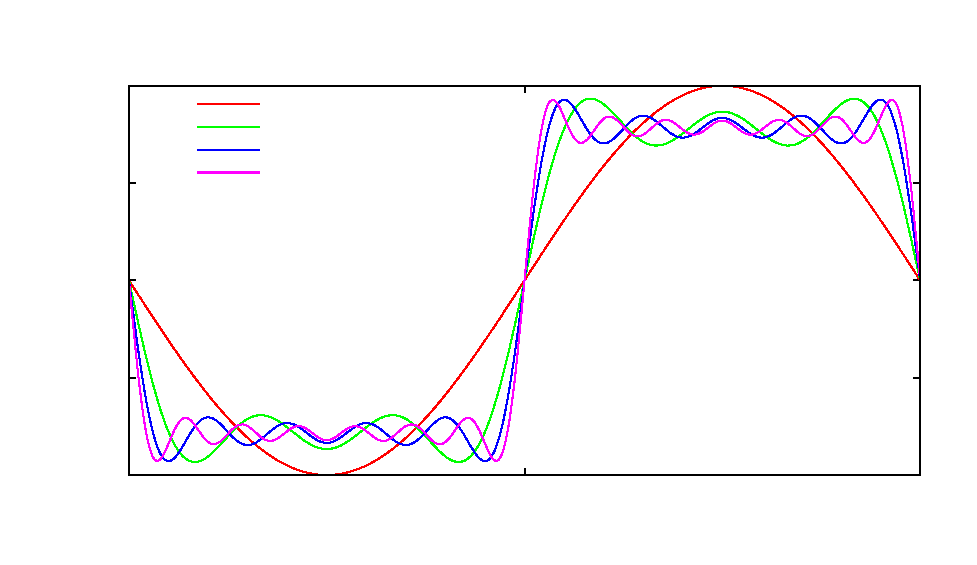
\includegraphics{Content/Intro/DummySection/Fouriersynthese/FourierOut}}%
    \gplfronttext
  \end{picture}%
\endgroup

	\caption{Eine Fouriersynthese}
	\label{fig:testfig}
\end{figure}

\bigskip
Und die dazu Passende Formel: \SeeEq{eq:fourier}
\index{Fouriersynthese}

\begin{equation}
	\sum_{i=0}^{n} \frac{1}{i \cdot 2 + 1} \cdot
	\sin \left( x \cdot \left( i \cdot 2 + 1 \right) \right)
	\label{eq:fourier}
\end{equation}

\clearpage
Und nun C++ Code: \SeeS{code:example}

\begin{c++}{Ein Stück Code}{code:example}
int main(int argc, char *argv[]) {
	int fd;
	int chars_sent;
	char buf[MAXBUF];

	if (argc < 3) {
		cerr << "argument missing, IP address an text needed, exiting..."<< endl;
		return 1;
	}

	/*
	 * multyrow comment
	 */

	// IP and Port
	sockaddr_in name;
	bzero(&name, sizeof(name));
	name.sin_family = AF_INET;
	inet_aton(argv[1], &(name.sin_addr));
	name.sin_port = htons(MYPORT);

	// connect to server
	DEBUG("try connect");
	if (connect(fd, (struct sockaddr *) &name, sizeof(name)) < 0) {
		PANIC("CONNECT");
	}
	// Transfer
	sprintf(buf, "%s:%s", argv[1], argv[2]);
	chars_sent = send(fd, buf, strlen(buf), 0);
	DEBUG("n=" << chars_sent << " Bytes sent");
	DEBUG("message length: " << strlen(buf));
	if (chars_sent < 0) {
		PANIC("SEND");
	}

	// close socket
	DEBUG("close socket");
	close(fd);

	return 0;
}
\end{c++}

Ein \index{Dummytext}Dummytext mit einer \ac{DUM} die öfter benutzt wird \ac{DUM}

\begin{longtable}{|c|m{12cm}|}
	\hline 
	Nummer & Anforderung \\
	\hline
	\EmptyRow 
	\hline \endhead
		\Textlabel{FA 1.1}{text:1} &
			Anforderung 1 \\
	\hline \Grayrow 
		\Textlabel{FA 1.2}{text:2} & 
			Anforderung 2\\ 
	\hline
	\CaptionLongtable{Funktionale Anforderungen an das Planungstool}
	\label{tab:FunctionalRequirements}
\end{longtable}

so kann darauf referenziert werden: \ref{text:1} \ref{text:2}

\chapter{Stand der Praxis}
\chapter{Eigene Ideen \& Konzepte}
\chapter{Methoden}
\chapter{Realisierung}
\chapter{Evaluation \& Validation}
\chapter{Ausblick}

%Appendix

\cleardoublepage
\phantomsection
\addcontentsline{toc}{chapter}{\listfigurename}
\listoffigures

\cleardoublepage
\phantomsection
\addcontentsline{toc}{chapter}{\listtablename}
\listoftables

\cleardoublepage
\phantomsection
\addcontentsline{toc}{chapter}{\lstlistlistingname}
\lstlistoflistings

\cleardoublepage
\phantomsection
\markboth{\uppercase{\ListOfAbbreviations}}{}
\chapter*{\ListOfAbbreviations}
\addcontentsline{toc}{chapter}{\ListOfAbbreviations}
%This is free and unencumbered software released into the public domain.
%
%Anyone is free to copy, modify, publish, use, compile, sell, or
%distribute this software, either in source code form or as a compiled
%binary, for any purpose, commercial or non-commercial, and by any
%means.
%
%In jurisdictions that recognize copyright laws, the author or authors
%of this software dedicate any and all copyright interest in the
%software to the public domain. We make this dedication for the benefit
%of the public at large and to the detriment of our heirs and
%successors. We intend this dedication to be an overt act of
%relinquishment in perpetuity of all present and future rights to this
%software under copyright law.
%
%THE SOFTWARE IS PROVIDED "AS IS", WITHOUT WARRANTY OF ANY KIND,
%EXPRESS OR IMPLIED, INCLUDING BUT NOT LIMITED TO THE WARRANTIES OF
%MERCHANTABILITY, FITNESS FOR A PARTICULAR PURPOSE AND NONINFRINGEMENT.
%IN NO EVENT SHALL THE AUTHORS BE LIABLE FOR ANY CLAIM, DAMAGES OR
%OTHER LIABILITY, WHETHER IN AN ACTION OF CONTRACT, TORT OR OTHERWISE,
%ARISING FROM, OUT OF OR IN CONNECTION WITH THE SOFTWARE OR THE USE OR
%OTHER DEALINGS IN THE SOFTWARE.
%
%For more information, please refer to <http://unlicense.org>


\setlength{\columnsep}{1 cm} % Space between columnseprule and right text
\setlength{\columnseprule}{\LineThickness} % Thikness of the columnseprule

\begin{multicols}{2}
	\begin{acronym}[wwwwwwwW] % The length of the longes abbreviation

		\renewcommand{\aclabelfont}[1]{\textbf{\textsf{#1}}\dotfill} % add dotfill
		\setlength{\itemsep}{1 pt} % set space between lines

		% another option to get the spacing right but it looks bad:
		% \centering

		% Sortet alphabetically by abbreviation
		\acro{DUM}{Dummy Abkürzung}
		\acro{USB}{Universal Serial Bus}
		\acro{LAN}{Local Area Network}
		\acro{UE4}{Unreal Enging 4}
	\end{acronym}
\end{multicols}

\cleardoublepage
\phantomsection
\addcontentsline{toc}{chapter}{\bibname}
\bibliography{BachelorthesisLiterature}

\cleardoublepage
\phantomsection
\addcontentsline{toc}{chapter}{\indexname}
\printindex

\thispagestyle{empty}
%This is free and unencumbered software released into the public domain.
%
%Anyone is free to copy, modify, publish, use, compile, sell, or
%distribute this software, either in source code form or as a compiled
%binary, for any purpose, commercial or non-commercial, and by any
%means.
%
%In jurisdictions that recognize copyright laws, the author or authors
%of this software dedicate any and all copyright interest in the
%software to the public domain. We make this dedication for the benefit
%of the public at large and to the detriment of our heirs and
%successors. We intend this dedication to be an overt act of
%relinquishment in perpetuity of all present and future rights to this
%software under copyright law.
%
%THE SOFTWARE IS PROVIDED "AS IS", WITHOUT WARRANTY OF ANY KIND,
%EXPRESS OR IMPLIED, INCLUDING BUT NOT LIMITED TO THE WARRANTIES OF
%MERCHANTABILITY, FITNESS FOR A PARTICULAR PURPOSE AND NONINFRINGEMENT.
%IN NO EVENT SHALL THE AUTHORS BE LIABLE FOR ANY CLAIM, DAMAGES OR
%OTHER LIABILITY, WHETHER IN AN ACTION OF CONTRACT, TORT OR OTHERWISE,
%ARISING FROM, OUT OF OR IN CONNECTION WITH THE SOFTWARE OR THE USE OR
%OTHER DEALINGS IN THE SOFTWARE.
%
%For more information, please refer to <http://unlicense.org>


{\ }
\vfill

\begin{flushleft}
%	SHORT ONE
%	Mit meiner Unterschrift bestätige ich, dass ich die Arbeit
%	selbstständig und nur mit den zugelassenen Hilfsmitteln erstellt habe.
	
	Hiermit erkläre ich, dass ich diese Bachelorarbeit selbstständig 
	angefertigt und keine anderen als die angegebenen Quellen und Hilfsmittel 
	benutzt habe. Alle wörtlich oder sinngemäß übernommenen Ausführungen wurden 
	als solche gekennzeichnet. Weiterhin erkläre ich, dass ich diese Arbeit in 
	gleicher oder ähnlicher Form nicht bereits einer anderen Prüfungsbehörde 
	vorgelegt habe.

%	TEXT FROM ASTA 
%	Ich erkläre hiermit an Eides statt, dass ich die vorliegende Arbeit 	
%	selbstständig und ohne unerlaubte fremde Hilfe angefertigt, andere als die 
%	angegebenen Quellen und Hilfsmittel nicht benutzt und die den benutzten 
%	Quellen wörtlich oder inhaltlich entnommenen Stellen als solche kenntlich 
%	gemacht habe.
%	
%	Dieser Datenträger dient der Vorlage bei dem/r Prüfer/in und der 
%	Prüfungskommission. Der Inhalt der Arbeit darf Dritten ohne ausdrückliche 
%	Genehmigung des Verfassers nicht zugänglich gemacht werden. Dies gilt 
%	insbesondere für die kommerzielle Nutzung, Server von Dritten oder die 
%	Überprüfung mit Hilfe von Plagiatssoftware.
\end{flushleft}

\vspace*{2cm}
\noindent{Minden, den \today ~ \dotfill}
\vspace*{4cm}

\end{document}